%!TEX root = YEAR-SURNAME-N-PhD.tex

\chapter{Results}\label{results}

We have a plot in Figure \ref{fig:plot} and more results in Table \ref{tab:table}.

\begin{figure}
\centering
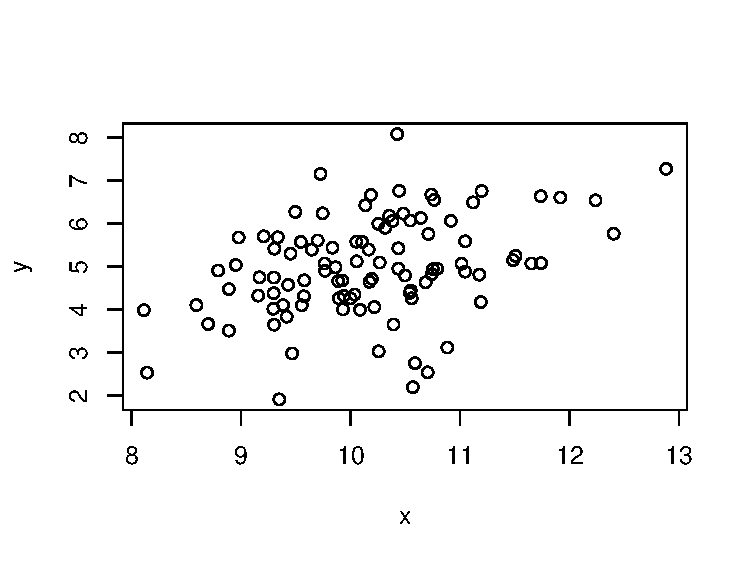
\includegraphics[width = 0.8\textwidth]{figures/plot-1}
\caption{Here goes a caption for this super-cool figure.}\label{fig:plot}
\end{figure}

\begin{table}
    \caption{\label{tab:table}Caption of the table.}
    \centering
    \begin{tabular}[t]{rr}
    \toprule
    x & y\\
    \midrule
    10.497248 & 4.796485\\
    9.301475 & 3.650826\\
    9.545996 & 5.576487\\
    10.686333 & 4.637482\\
    10.426642 & 8.084386\\
    10.086181 & 3.999149\\
    \bottomrule
    \end{tabular}
\end{table}
